\subsection{ブラジル領域における解析結果}
\label{sec:result_brazil}

\subsubsection{データセット}
ブラジル領域において表\ref{tab:station_info_br}に示す2つの観測点のデータを用いた。

\begin{table}[htbp]
  \centering
  \caption{ブラジル領域の観測点情報}
  \label{tab:station_info_br}
  \begin{tabular}{llccc}
    \toprule
    Code & Name & Nation & Dip Lat & Long \\
    \midrule
    TTB & Tatuoca & Brazil & $0.20^\circ$ & $-48.51^\circ$ \\
    EUS & Eusebio & Brazil & $-9.41^\circ$ & $-38.43^\circ$ \\
    \bottomrule
  \end{tabular}
\end{table}

TTBは磁気赤道上（Dip equator）、EUSは磁気赤道から離れた低緯度地域（Offdip equator）に位置している。
なお、本解析におけるDip観測点とOffdip観測点間のEUELの相関係数の閾値は0.55に設定した。

\subsubsection{季節依存性}
未発達型と突発型の月ごとの発生割合を図\ref{fig:undeveloped_monthly}、図\ref{fig:sudden_monthly}に示す。

\begin{figure}[htbp]
  \centering
  \begin{minipage}{0.48\linewidth}
    \centering
    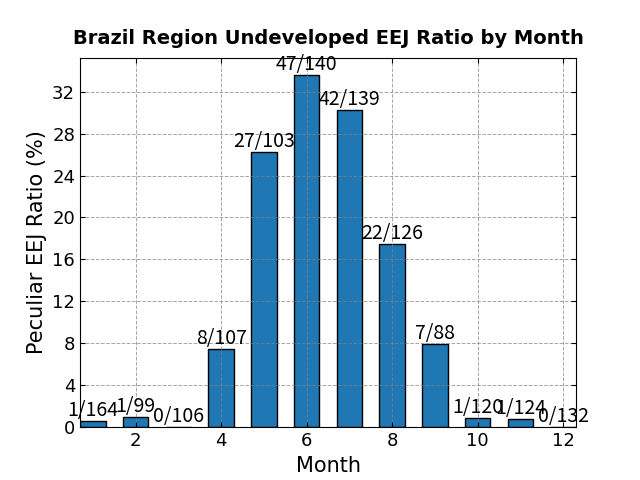
\includegraphics[width=\linewidth]{figures/2009-2020_brazil_undeveloped_month.png}
    \caption{未発達型EEJの月ごとの発生割合（2009-2020年）}
    \label{fig:undeveloped_monthly}
  \end{minipage}
  \hfill
  \begin{minipage}{0.48\linewidth}
    \centering
    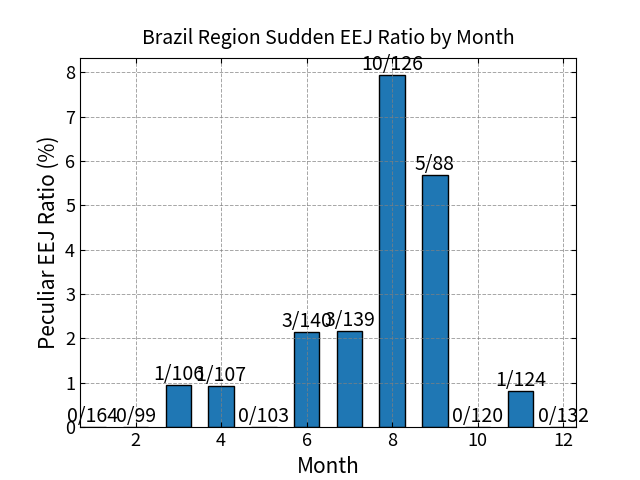
\includegraphics[width=\linewidth]{figures/2009-2020_brazil_sudden_month.png}
    \caption{突発型EEJの月ごとの発生割合（2009-2020年）}
    \label{fig:sudden_monthly}
  \end{minipage}
\end{figure}

解析の結果、未発達型は南半球の冬至にあたるJ-solstice（5月〜7月）において、発生率が特に高い傾向を示した。
具体的には、5月に103件中27件、6月に140件中47件、7月に139件中42件発生し、この期間の発生率のピークは約33\%であった。
対照的に、夏至にあたるD-solstice（10月〜2月）においては、発生率が著しく低下した。
具体的には、10月は120件中1件、11月は124件中1件、12月は132件中0件、1月は164件中1件、2月は99件中1件であり、発生率は約1\%に留まった。

突発型においては、9月と10月に発生率が高い傾向を示した。
具体的には、9月に126件中10件、10月に88件中5件発生し、発生率は約8\%であった。
一方で、それ以外の月は発生率が低く、いずれも2\%以下であった。

\subsubsection{月潮汐効果との対応関係}
未発達型と突発型の月齢ごとの発生割合を図\ref{fig:undeveloped_lunar}、図\ref{fig:sudden_lunar}に示す。

\begin{figure}[htbp]
  \centering
  \begin{minipage}{0.48\linewidth}
    \centering
    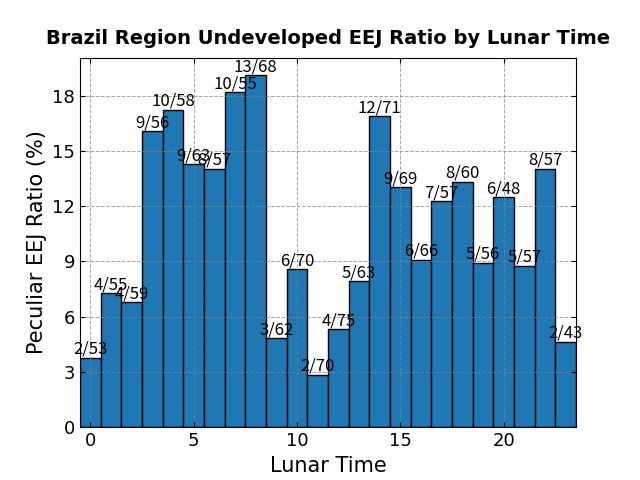
\includegraphics[width=\linewidth]{figures/2009-2020_brazil_undeveloped_lunar.png}
    \caption{未発達型EEJの月齢ごとの発生割合（2009-2020年）}
    \label{fig:undeveloped_lunar}
  \end{minipage}
  \hfill
  \begin{minipage}{0.48\linewidth}
    \centering
    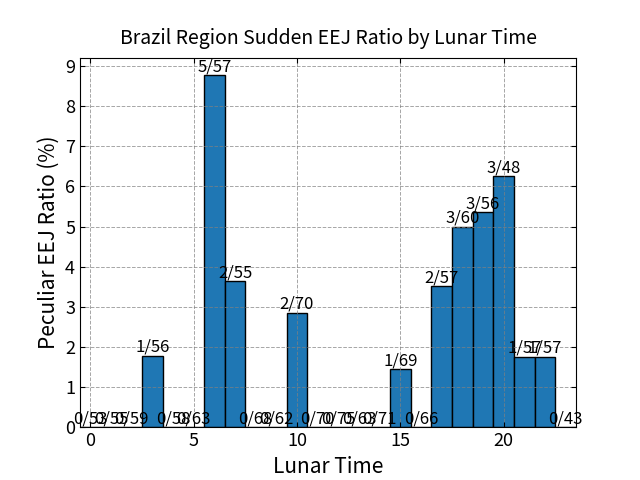
\includegraphics[width=\linewidth]{figures/2009-2020_brazil_sudden_lunar.png}
    \caption{突発型EEJの月齢ごとの発生割合（2009-2020年）}
    \label{fig:sudden_lunar}
  \end{minipage}
\end{figure}

解析の結果、未発達型においては、Lunar age = 3--8で発生率が約18\%と最も高く、次いでLunar age = 14--22で約12\%のピークが確認された。
一方、Lunar age = 0--2および9--13では発生率が低い傾向が見られた。

突発型においては、Lunar age = 6--7で発生率が最も高く、次いでLunar age = 17--20で高い傾向が見られた。
一方、Lunar age = 0--5, 8--16, 21--24では発生率が極めて低く、発生数が0件または1件のケースが大半を占めた。